\documentclass[10pt,a4paper]{article}
\usepackage{amsmath,amssymb,amsthm,graphicx}
\usepackage{mathtools,stmaryrd,mathrsfs,wasysym,xspace,enumitem,etoolbox,aliascnt,hyperref,cleveref,braket}
\usepackage[all,2cell,cmtip]{xy}
\UseAllTwocells
\usepackage{tikz}
\usetikzlibrary{decorations.pathmorphing,arrows}
\newcounter{chapter}
\renewcommand{\thesection}{\thechapter.\arabic{section}}
\providecommand{\index}[1]{}
%%%% MACROS FOR NOTATION %%%%
% Use these for any notation where there are multiple options.

%%% Notes and exercise sections
\makeatletter
\newcommand{\sectionNotes}{\phantomsection\section*{Notes}\addcontentsline{toc}{section}{Notes}\markright{\textsc{\@chapapp{} \thechapter{} Notes}}}
\newcommand{\sectionExercises}[1]{\ifdef{\OPTexerciseperpage}{\newpage}{}\phantomsection\section*{Exercises}\addcontentsline{toc}{section}{Exercises}\markright{\textsc{\@chapapp{} \thechapter{} Exercises}}}
\makeatother

%%% Definitional equality (used infix) %%%
\newcommand{\jdeq}{\equiv}      % An equality judgment
\let\judgeq\jdeq
%\newcommand{\defeq}{\coloneqq}  % An equality currently being defined
\newcommand{\defeq}{\vcentcolon\equiv}  % A judgmental equality currently being defined

%%% Term being defined
\newcommand{\define}[1]{\textbf{#1}}

%%% Vec (for example)

\newcommand{\Vect}{\ensuremath{\mathsf{Vec}}}
\newcommand{\Fin}{\ensuremath{\mathsf{Fin}}}
\newcommand{\fmax}{\ensuremath{\mathsf{fmax}}}
\newcommand{\seq}[1]{\langle #1\rangle}

%%% Dependent products %%%
\def\prdsym{\textstyle\prod}
%% Call the macro like \prd{x,y:A}{p:x=y} with any number of
%% arguments.  Make sure that whatever comes *after* the call doesn't
%% begin with an open-brace, or it will be parsed as another argument.
\makeatletter
% Currently the macro is configured to produce
%     {\textstyle\prod}(x:A) \; {\textstyle\prod}(y:B),{\ }
% in display-math mode, and
%     \prod_{(x:A)} \prod_{y:B}
% in text-math mode.
% \def\prd#1{\@ifnextchar\bgroup{\prd@parens{#1}}{%
%     \@ifnextchar\sm{\prd@parens{#1}\@eatsm}{%
%         \prd@noparens{#1}}}}
\def\prd#1{\@ifnextchar\bgroup{\prd@parens{#1}}{%
    \@ifnextchar\sm{\prd@parens{#1}\@eatsm}{%
    \@ifnextchar\prd{\prd@parens{#1}\@eatprd}{%
    \@ifnextchar\;{\prd@parens{#1}\@eatsemicolonspace}{%
    \@ifnextchar\\{\prd@parens{#1}\@eatlinebreak}{%
    \@ifnextchar\narrowbreak{\prd@parens{#1}\@eatnarrowbreak}{%
      \prd@noparens{#1}}}}}}}}
\def\prd@parens#1{\@ifnextchar\bgroup%
  {\mathchoice{\@dprd{#1}}{\@tprd{#1}}{\@tprd{#1}}{\@tprd{#1}}\prd@parens}%
  {\@ifnextchar\sm%
    {\mathchoice{\@dprd{#1}}{\@tprd{#1}}{\@tprd{#1}}{\@tprd{#1}}\@eatsm}%
    {\mathchoice{\@dprd{#1}}{\@tprd{#1}}{\@tprd{#1}}{\@tprd{#1}}}}}
\def\@eatsm\sm{\sm@parens}
\def\prd@noparens#1{\mathchoice{\@dprd@noparens{#1}}{\@tprd{#1}}{\@tprd{#1}}{\@tprd{#1}}}
% Helper macros for three styles
\def\lprd#1{\@ifnextchar\bgroup{\@lprd{#1}\lprd}{\@@lprd{#1}}}
\def\@lprd#1{\mathchoice{{\textstyle\prod}}{\prod}{\prod}{\prod}({\textstyle #1})\;}
\def\@@lprd#1{\mathchoice{{\textstyle\prod}}{\prod}{\prod}{\prod}({\textstyle #1}),\ }
\def\tprd#1{\@tprd{#1}\@ifnextchar\bgroup{\tprd}{}}
\def\@tprd#1{\mathchoice{{\textstyle\prod_{(#1)}}}{\prod_{(#1)}}{\prod_{(#1)}}{\prod_{(#1)}}}
\def\dprd#1{\@dprd{#1}\@ifnextchar\bgroup{\dprd}{}}
\def\@dprd#1{\prod_{(#1)}\,}
\def\@dprd@noparens#1{\prod_{#1}\,}

% Look through spaces and linebreaks
\def\@eatnarrowbreak\narrowbreak{%
  \@ifnextchar\prd{\narrowbreak\@eatprd}{%
    \@ifnextchar\sm{\narrowbreak\@eatsm}{%
      \narrowbreak}}}
\def\@eatlinebreak\\{%
  \@ifnextchar\prd{\\\@eatprd}{%
    \@ifnextchar\sm{\\\@eatsm}{%
      \\}}}
\def\@eatsemicolonspace\;{%
  \@ifnextchar\prd{\;\@eatprd}{%
    \@ifnextchar\sm{\;\@eatsm}{%
      \;}}}

%%% Lambda abstractions.
% Each variable being abstracted over is a separate argument.  If
% there is more than one such argument, they *must* be enclosed in
% braces.  Arguments can be untyped, as in \lam{x}{y}, or typed with a
% colon, as in \lam{x:A}{y:B}. In the latter case, the colons are
% automatically noticed and (with current implementation) the space
% around the colon is reduced.  You can even give more than one variable
% the same type, as in \lam{x,y:A}.
\def\lam#1{{\lambda}\@lamarg#1:\@endlamarg\@ifnextchar\bgroup{.\,\lam}{.\,}}
\def\@lamarg#1:#2\@endlamarg{\if\relax\detokenize{#2}\relax #1\else\@lamvar{\@lameatcolon#2},#1\@endlamvar\fi}
\def\@lamvar#1,#2\@endlamvar{(#2\,{:}\,#1)}
% \def\@lamvar#1,#2{{#2}^{#1}\@ifnextchar,{.\,{\lambda}\@lamvar{#1}}{\let\@endlamvar\relax}}
\def\@lameatcolon#1:{#1}
\let\lamt\lam
% This version silently eats any typing annotation.
\def\lamu#1{{\lambda}\@lamuarg#1:\@endlamuarg\@ifnextchar\bgroup{.\,\lamu}{.\,}}
\def\@lamuarg#1:#2\@endlamuarg{#1}

%%% Dependent products written with \forall, in the same style
\def\fall#1{\forall (#1)\@ifnextchar\bgroup{.\,\fall}{.\,}}

%%% Existential quantifier %%%
\def\exis#1{\exists (#1)\@ifnextchar\bgroup{.\,\exis}{.\,}}

%%% Dependent sums %%%
\def\smsym{\textstyle\sum}
% Use in the same way as \prd
\def\sm#1{\@ifnextchar\bgroup{\sm@parens{#1}}{%
    \@ifnextchar\prd{\sm@parens{#1}\@eatprd}{%
    \@ifnextchar\sm{\sm@parens{#1}\@eatsm}{%
    \@ifnextchar\;{\sm@parens{#1}\@eatsemicolonspace}{%
    \@ifnextchar\\{\sm@parens{#1}\@eatlinebreak}{%
    \@ifnextchar\narrowbreak{\sm@parens{#1}\@eatnarrowbreak}{%
        \sm@noparens{#1}}}}}}}}
\def\sm@parens#1{\@ifnextchar\bgroup%
  {\mathchoice{\@dsm{#1}}{\@tsm{#1}}{\@tsm{#1}}{\@tsm{#1}}\sm@parens}%
  {\@ifnextchar\prd%
    {\mathchoice{\@dsm{#1}}{\@tsm{#1}}{\@tsm{#1}}{\@tsm{#1}}\@eatprd}%
    {\mathchoice{\@dsm{#1}}{\@tsm{#1}}{\@tsm{#1}}{\@tsm{#1}}}}}
\def\@eatprd\prd{\prd@parens}
\def\sm@noparens#1{\mathchoice{\@dsm@noparens{#1}}{\@tsm{#1}}{\@tsm{#1}}{\@tsm{#1}}}
\def\lsm#1{\@ifnextchar\bgroup{\@lsm{#1}\lsm}{\@@lsm{#1}}}
\def\@lsm#1{\mathchoice{{\textstyle\sum}}{\sum}{\sum}{\sum}({\textstyle #1})\;}
\def\@@lsm#1{\mathchoice{{\textstyle\sum}}{\sum}{\sum}{\sum}({\textstyle #1}),\ }
\def\tsm#1{\@tsm{#1}\@ifnextchar\bgroup{\tsm}{}}
\def\@tsm#1{\mathchoice{{\textstyle\sum_{(#1)}}}{\sum_{(#1)}}{\sum_{(#1)}}{\sum_{(#1)}}}
\def\dsm#1{\@dsm{#1}\@ifnextchar\bgroup{\dsm}{}}
\def\@dsm#1{\sum_{(#1)}\,}
\def\@dsm@noparens#1{\sum_{#1}\,}

%%% W-types
\def\wtypesym{{\mathsf{W}}}
\def\wtype#1{\@ifnextchar\bgroup%
  {\mathchoice{\@twtype{#1}}{\@twtype{#1}}{\@twtype{#1}}{\@twtype{#1}}\wtype}%
  {\mathchoice{\@twtype{#1}}{\@twtype{#1}}{\@twtype{#1}}{\@twtype{#1}}}}
\def\lwtype#1{\@ifnextchar\bgroup{\@lwtype{#1}\lwtype}{\@@lwtype{#1}}}
\def\@lwtype#1{\mathchoice{{\textstyle\mathsf{W}}}{\mathsf{W}}{\mathsf{W}}{\mathsf{W}}({\textstyle #1})\;}
\def\@@lwtype#1{\mathchoice{{\textstyle\mathsf{W}}}{\mathsf{W}}{\mathsf{W}}{\mathsf{W}}({\textstyle #1}),\ }
\def\twtype#1{\@twtype{#1}\@ifnextchar\bgroup{\twtype}{}}
\def\@twtype#1{\mathchoice{{\textstyle\mathsf{W}_{(#1)}}}{\mathsf{W}_{(#1)}}{\mathsf{W}_{(#1)}}{\mathsf{W}_{(#1)}}}
\def\dwtype#1{\@dwtype{#1}\@ifnextchar\bgroup{\dwtype}{}}
\def\@dwtype#1{\mathsf{W}_{(#1)}\,}

\newcommand{\suppsym}{{\mathsf{sup}}}
\newcommand{\supp}{\ensuremath\suppsym\xspace}

\def\wtypeh#1{\@ifnextchar\bgroup%
  {\mathchoice{\@lwtypeh{#1}}{\@twtypeh{#1}}{\@twtypeh{#1}}{\@twtypeh{#1}}\wtypeh}%
  {\mathchoice{\@@lwtypeh{#1}}{\@twtypeh{#1}}{\@twtypeh{#1}}{\@twtypeh{#1}}}}
\def\lwtypeh#1{\@ifnextchar\bgroup{\@lwtypeh{#1}\lwtypeh}{\@@lwtypeh{#1}}}
\def\@lwtypeh#1{\mathchoice{{\textstyle\mathsf{W}^h}}{\mathsf{W}^h}{\mathsf{W}^h}{\mathsf{W}^h}({\textstyle #1})\;}
\def\@@lwtypeh#1{\mathchoice{{\textstyle\mathsf{W}^h}}{\mathsf{W}^h}{\mathsf{W}^h}{\mathsf{W}^h}({\textstyle #1}),\ }
\def\twtypeh#1{\@twtypeh{#1}\@ifnextchar\bgroup{\twtypeh}{}}
\def\@twtypeh#1{\mathchoice{{\textstyle\mathsf{W}^h_{(#1)}}}{\mathsf{W}^h_{(#1)}}{\mathsf{W}^h_{(#1)}}{\mathsf{W}^h_{(#1)}}}
\def\dwtypeh#1{\@dwtypeh{#1}\@ifnextchar\bgroup{\dwtypeh}{}}
\def\@dwtypeh#1{\mathsf{W}^h_{(#1)}\,}


\makeatother

% Other notations related to dependent sums
\let\setof\Set    % from package 'braket', write \setof{ x:A | P(x) }.
\newcommand{\pair}{\ensuremath{\mathsf{pair}}\xspace}
\newcommand{\tup}[2]{(#1,#2)}
\newcommand{\proj}[1]{\ensuremath{\mathsf{pr}_{#1}}\xspace}
\newcommand{\fst}{\ensuremath{\proj1}\xspace}
\newcommand{\snd}{\ensuremath{\proj2}\xspace}
\newcommand{\ac}{\ensuremath{\mathsf{ac}}\xspace} % not needed in symbol index

%%% recursor and induction
\newcommand{\rec}[1]{\mathsf{rec}_{#1}}
\newcommand{\ind}[1]{\mathsf{ind}_{#1}}
\newcommand{\indid}[1]{\ind{=_{#1}}} % (Martin-Lof) path induction principle for identity types
\newcommand{\indidb}[1]{\ind{=_{#1}}'} % (Paulin-Mohring) based path induction principle for identity types

%%% Uniqueness principles
\newcommand{\uniq}[1]{\mathsf{uniq}_{#1}}

% Paths in pairs
\newcommand{\pairpath}{\ensuremath{\mathsf{pair}^{\mathord{=}}}\xspace}
% \newcommand{\projpath}[1]{\proj{#1}^{\mathord{=}}}
\newcommand{\projpath}[1]{\ensuremath{\apfunc{\proj{#1}}}\xspace}
\newcommand{\pairct}{\ensuremath{\mathsf{pair}^{\mathord{\ct}}}\xspace}

%%% For quotients %%%
%\newcommand{\pairr}[1]{{\langle #1\rangle}}
\newcommand{\pairr}[1]{{\mathopen{}(#1)\mathclose{}}}
\newcommand{\Pairr}[1]{{\mathopen{}\left(#1\right)\mathclose{}}}

% \newcommand{\type}{\ensuremath{\mathsf{Type}}} % this command is overridden below, so it's commented out
\newcommand{\im}{\ensuremath{\mathsf{im}}} % the image

%%% 2D path operations
\newcommand{\leftwhisker}{\mathbin{{\ct}_{\mathsf{l}}}}  % was \ell
\newcommand{\rightwhisker}{\mathbin{{\ct}_{\mathsf{r}}}} % was r
\newcommand{\hct}{\star}

%%% modalities %%%
\newcommand{\modal}{\ensuremath{\ocircle}}
\let\reflect\modal
\newcommand{\modaltype}{\ensuremath{\type_\modal}}
% \newcommand{\ism}[1]{\ensuremath{\mathsf{is}_{#1}}}
% \newcommand{\ismodal}{\ism{\modal}}
% \newcommand{\existsmodal}{\ensuremath{{\exists}_{\modal}}}
% \newcommand{\existsmodalunique}{\ensuremath{{\exists!}_{\modal}}}
% \newcommand{\modalfunc}{\textsf{\modal-fun}}
% \newcommand{\Ecirc}{\ensuremath{\mathsf{E}_\modal}}
% \newcommand{\Mcirc}{\ensuremath{\mathsf{M}_\modal}}
\newcommand{\mreturn}{\ensuremath{\eta}}
\let\project\mreturn
%\newcommand{\mbind}[1]{\ensuremath{\hat{#1}}}
\newcommand{\ext}{\mathsf{ext}}
%\newcommand{\mmap}[1]{\ensuremath{\bar{#1}}}
%\newcommand{\mjoin}{\ensuremath{\mreturn^{-1}}}
% Subuniverse
\renewcommand{\P}{\ensuremath{\type_{P}}\xspace}

%%% Localizations
% \newcommand{\islocal}[1]{\ensuremath{\mathsf{islocal}_{#1}}\xspace}
% \newcommand{\loc}[1]{\ensuremath{\mathcal{L}_{#1}}\xspace}

%%% Identity types %%%
\newcommand{\idsym}{{=}}
\newcommand{\id}[3][]{\ensuremath{#2 =_{#1} #3}\xspace}
\newcommand{\idtype}[3][]{\ensuremath{\mathsf{Id}_{#1}(#2,#3)}\xspace}
\newcommand{\idtypevar}[1]{\ensuremath{\mathsf{Id}_{#1}}\xspace}
% A propositional equality currently being defined
\newcommand{\defid}{\coloneqq}

%%% Dependent paths
\newcommand{\dpath}[4]{#3 =^{#1}_{#2} #4}

%%% singleton
% \newcommand{\sgl}{\ensuremath{\mathsf{sgl}}\xspace}
% \newcommand{\sctr}{\ensuremath{\mathsf{sctr}}\xspace}

%%% Reflexivity terms %%%
% \newcommand{\reflsym}{{\mathsf{refl}}}
\newcommand{\refl}[1]{\ensuremath{\mathsf{refl}_{#1}}\xspace}

%%% Path concatenation (used infix, in diagrammatic order) %%%
\newcommand{\ct}{%
  \mathchoice{\mathbin{\raisebox{0.5ex}{$\displaystyle\centerdot$}}}%
             {\mathbin{\raisebox{0.5ex}{$\centerdot$}}}%
             {\mathbin{\raisebox{0.25ex}{$\scriptstyle\,\centerdot\,$}}}%
             {\mathbin{\raisebox{0.1ex}{$\scriptscriptstyle\,\centerdot\,$}}}
}

%%% Path reversal %%%
\newcommand{\opp}[1]{\mathord{{#1}^{-1}}}
\let\rev\opp

%%% Coherence paths %%%
\newcommand{\ctassoc}{\mathsf{assoc}} % associativity law

%%% Transport (covariant) %%%
\newcommand{\trans}[2]{\ensuremath{{#1}_{*}\mathopen{}\left({#2}\right)\mathclose{}}\xspace}
\let\Trans\trans
%\newcommand{\Trans}[2]{\ensuremath{{#1}_{*}\left({#2}\right)}\xspace}
\newcommand{\transf}[1]{\ensuremath{{#1}_{*}}\xspace} % Without argument
%\newcommand{\transport}[2]{\ensuremath{\mathsf{transport}_{*} \: {#2}\xspace}}
\newcommand{\transfib}[3]{\ensuremath{\mathsf{transport}^{#1}(#2,#3)\xspace}}
\newcommand{\Transfib}[3]{\ensuremath{\mathsf{transport}^{#1}\Big(#2,\, #3\Big)\xspace}}
\newcommand{\transfibf}[1]{\ensuremath{\mathsf{transport}^{#1}\xspace}}

%%% 2D transport
\newcommand{\transtwo}[2]{\ensuremath{\mathsf{transport}^2\mathopen{}\left({#1},{#2}\right)\mathclose{}}\xspace}

%%% Constant transport
\newcommand{\transconst}[3]{\ensuremath{\mathsf{transportconst}}^{#1}_{#2}(#3)\xspace}
\newcommand{\transconstf}{\ensuremath{\mathsf{transportconst}}\xspace}

%%% Map on paths %%%
\newcommand{\mapfunc}[1]{\ensuremath{\mathsf{ap}_{#1}}\xspace} % Without argument
\newcommand{\map}[2]{\ensuremath{{#1}\mathopen{}\left({#2}\right)\mathclose{}}\xspace}
\let\Ap\map
%\newcommand{\Ap}[2]{\ensuremath{{#1}\left({#2}\right)}\xspace}
\newcommand{\mapdepfunc}[1]{\ensuremath{\mathsf{apd}_{#1}}\xspace} % Without argument
% \newcommand{\mapdep}[2]{\ensuremath{{#1}\llparenthesis{#2}\rrparenthesis}\xspace}
\newcommand{\mapdep}[2]{\ensuremath{\mapdepfunc{#1}\mathopen{}\left(#2\right)\mathclose{}}\xspace}
\let\apfunc\mapfunc
\let\ap\map
\let\apdfunc\mapdepfunc
\let\apd\mapdep

%%% 2D map on paths
\newcommand{\aptwofunc}[1]{\ensuremath{\mathsf{ap}^2_{#1}}\xspace}
\newcommand{\aptwo}[2]{\ensuremath{\aptwofunc{#1}\mathopen{}\left({#2}\right)\mathclose{}}\xspace}
\newcommand{\apdtwofunc}[1]{\ensuremath{\mathsf{apd}^2_{#1}}\xspace}
\newcommand{\apdtwo}[2]{\ensuremath{\apdtwofunc{#1}\mathopen{}\left(#2\right)\mathclose{}}\xspace}

%%% Identity functions %%%
\newcommand{\idfunc}[1][]{\ensuremath{\mathsf{id}_{#1}}\xspace}

%%% Homotopies (written infix) %%%
\newcommand{\htpy}{\sim}

%%% Other meanings of \sim
\newcommand{\bisim}{\sim}       % bisimulation
\newcommand{\eqr}{\sim}         % an equivalence relation

%%% Equivalence types %%%
\newcommand{\eqv}[2]{\ensuremath{#1 \simeq #2}\xspace}
\newcommand{\eqvspaced}[2]{\ensuremath{#1 \;\simeq\; #2}\xspace}
\newcommand{\eqvsym}{\simeq}    % infix symbol
\newcommand{\texteqv}[2]{\ensuremath{\mathsf{Equiv}(#1,#2)}\xspace}
\newcommand{\isequiv}{\ensuremath{\mathsf{isequiv}}}
\newcommand{\qinv}{\ensuremath{\mathsf{qinv}}}
\newcommand{\ishae}{\ensuremath{\mathsf{ishae}}}
\newcommand{\linv}{\ensuremath{\mathsf{linv}}}
\newcommand{\rinv}{\ensuremath{\mathsf{rinv}}}
\newcommand{\biinv}{\ensuremath{\mathsf{biinv}}}
\newcommand{\lcoh}[3]{\mathsf{lcoh}_{#1}(#2,#3)}
\newcommand{\rcoh}[3]{\mathsf{rcoh}_{#1}(#2,#3)}
\newcommand{\hfib}[2]{{\mathsf{fib}}_{#1}(#2)}

%%% Map on total spaces %%%
\newcommand{\total}[1]{\ensuremath{\mathsf{total}(#1)}}

%%% Universe types %%%
%\newcommand{\type}{\ensuremath{\mathsf{Type}}\xspace}
\newcommand{\UU}{\ensuremath{\mathcal{U}}\xspace}
\let\bbU\UU
\let\type\UU
% Universes of truncated types
\newcommand{\typele}[1]{\ensuremath{{#1}\text-\mathsf{Type}}\xspace}
\newcommand{\typeleU}[1]{\ensuremath{{#1}\text-\mathsf{Type}_\UU}\xspace}
\newcommand{\typelep}[1]{\ensuremath{{(#1)}\text-\mathsf{Type}}\xspace}
\newcommand{\typelepU}[1]{\ensuremath{{(#1)}\text-\mathsf{Type}_\UU}\xspace}
\let\ntype\typele
\let\ntypeU\typeleU
\let\ntypep\typelep
\let\ntypepU\typelepU
\renewcommand{\set}{\ensuremath{\mathsf{Set}}\xspace}
\newcommand{\setU}{\ensuremath{\mathsf{Set}_\UU}\xspace}
\newcommand{\prop}{\ensuremath{\mathsf{Prop}}\xspace}
\newcommand{\propU}{\ensuremath{\mathsf{Prop}_\UU}\xspace}
%Pointed types
\newcommand{\pointed}[1]{\ensuremath{#1_\bullet}}

%%% Ordinals and cardinals
\newcommand{\card}{\ensuremath{\mathsf{Card}}\xspace}
\newcommand{\ord}{\ensuremath{\mathsf{Ord}}\xspace}
\newcommand{\ordsl}[2]{{#1}_{/#2}}

%%% Univalence
\newcommand{\ua}{\ensuremath{\mathsf{ua}}\xspace} % the inverse of idtoeqv
\newcommand{\idtoeqv}{\ensuremath{\mathsf{idtoeqv}}\xspace}
\newcommand{\univalence}{\ensuremath{\mathsf{univalence}}\xspace} % the full axiom

%%% Truncation levels
\newcommand{\iscontr}{\ensuremath{\mathsf{isContr}}}
\newcommand{\contr}{\ensuremath{\mathsf{contr}}} % The path to the center of contraction
\newcommand{\isset}{\ensuremath{\mathsf{isSet}}}
\newcommand{\isprop}{\ensuremath{\mathsf{isProp}}}
% h-propositions
% \newcommand{\anhprop}{a mere proposition\xspace}
% \newcommand{\hprops}{mere propositions\xspace}

%%% Homotopy fibers %%%
%\newcommand{\hfiber}[2]{\ensuremath{\mathsf{hFiber}(#1,#2)}\xspace}
\let\hfiber\hfib

%%% Bracket/squash/truncation types %%%
% \newcommand{\brck}[1]{\textsf{mere}(#1)}
% \newcommand{\Brck}[1]{\textsf{mere}\Big(#1\Big)}
% \newcommand{\trunc}[2]{\tau_{#1}(#2)}
% \newcommand{\Trunc}[2]{\tau_{#1}\Big(#2\Big)}
% \newcommand{\truncf}[1]{\tau_{#1}}
%\newcommand{\trunc}[2]{\Vert #2\Vert_{#1}}
\newcommand{\trunc}[2]{\mathopen{}\left\Vert #2\right\Vert_{#1}\mathclose{}}
\newcommand{\ttrunc}[2]{\bigl\Vert #2\bigr\Vert_{#1}}
\newcommand{\Trunc}[2]{\Bigl\Vert #2\Bigr\Vert_{#1}}
\newcommand{\truncf}[1]{\Vert \blank \Vert_{#1}}
\newcommand{\tproj}[3][]{\mathopen{}\left|#3\right|_{#2}^{#1}\mathclose{}}
\newcommand{\tprojf}[2][]{|\blank|_{#2}^{#1}}
\def\pizero{\trunc0}
%\newcommand{\brck}[1]{\trunc{-1}{#1}}
%\newcommand{\Brck}[1]{\Trunc{-1}{#1}}
%\newcommand{\bproj}[1]{\tproj{-1}{#1}}
%\newcommand{\bprojf}{\tprojf{-1}}

\newcommand{\brck}[1]{\trunc{}{#1}}
\newcommand{\bbrck}[1]{\ttrunc{}{#1}}
\newcommand{\Brck}[1]{\Trunc{}{#1}}
\newcommand{\bproj}[1]{\tproj{}{#1}}
\newcommand{\bprojf}{\tprojf{}}

% Big parentheses
\newcommand{\Parens}[1]{\Bigl(#1\Bigr)}

% Projection and extension for truncations
\let\extendsmb\ext
\newcommand{\extend}[1]{\extendsmb(#1)}

%
%%% The empty type
\newcommand{\emptyt}{\ensuremath{\mathbf{0}}\xspace}

%%% The unit type
\newcommand{\unit}{\ensuremath{\mathbf{1}}\xspace}
\newcommand{\ttt}{\ensuremath{\star}\xspace}

%%% The two-element type
\newcommand{\bool}{\ensuremath{\mathbf{2}}\xspace}
\newcommand{\btrue}{{1_{\bool}}}
\newcommand{\bfalse}{{0_{\bool}}}

%%% Injections into binary sums and pushouts
\newcommand{\inlsym}{{\mathsf{inl}}}
\newcommand{\inrsym}{{\mathsf{inr}}}
\newcommand{\inl}{\ensuremath\inlsym\xspace}
\newcommand{\inr}{\ensuremath\inrsym\xspace}

%%% The segment of the interval
\newcommand{\seg}{\ensuremath{\mathsf{seg}}\xspace}

%%% Free groups
\newcommand{\freegroup}[1]{F(#1)}
\newcommand{\freegroupx}[1]{F'(#1)} % the "other" free group

%%% Glue of a pushout
\newcommand{\glue}{\mathsf{glue}}

%%% Colimits
\newcommand{\colim}{\mathsf{colim}}
\newcommand{\inc}{\mathsf{inc}}
\newcommand{\cmp}{\mathsf{cmp}}

%%% Circles and spheres
\newcommand{\Sn}{\mathbb{S}}
\newcommand{\base}{\ensuremath{\mathsf{base}}\xspace}
\newcommand{\lloop}{\ensuremath{\mathsf{loop}}\xspace}
\newcommand{\surf}{\ensuremath{\mathsf{surf}}\xspace}

%%% Suspension
\newcommand{\susp}{\Sigma}
\newcommand{\north}{\mathsf{N}}
\newcommand{\south}{\mathsf{S}}
\newcommand{\merid}{\mathsf{merid}}

%%% Blanks (shorthand for lambda abstractions)
\newcommand{\blank}{\mathord{\hspace{1pt}\text{--}\hspace{1pt}}}

%%% Nameless objects
\newcommand{\nameless}{\mathord{\hspace{1pt}\underline{\hspace{1ex}}\hspace{1pt}}}

%%% Some decorations
%\newcommand{\bbU}{\ensuremath{\mathbb{U}}\xspace}
% \newcommand{\bbB}{\ensuremath{\mathbb{B}}\xspace}
\newcommand{\bbP}{\ensuremath{\mathbb{P}}\xspace}

%%% Some categories
\newcommand{\uset}{\ensuremath{\mathcal{S}et}\xspace}
\newcommand{\ucat}{\ensuremath{{\mathcal{C}at}}\xspace}
\newcommand{\urel}{\ensuremath{\mathcal{R}el}\xspace}
\newcommand{\uhilb}{\ensuremath{\mathcal{H}ilb}\xspace}
\newcommand{\utype}{\ensuremath{\mathcal{T}\!ype}\xspace}

% Pullback corner
\newbox\pbbox
\setbox\pbbox=\hbox{\xy \POS(65,0)\ar@{-} (0,0) \ar@{-} (65,65)\endxy}
\def\pb{\save[]+<3.5mm,-3.5mm>*{\copy\pbbox} \restore}

% Macros for the categories chapter
\newcommand{\inv}[1]{{#1}^{-1}}
\newcommand{\idtoiso}{\ensuremath{\mathsf{idtoiso}}\xspace}
\newcommand{\isotoid}{\ensuremath{\mathsf{isotoid}}\xspace}
\newcommand{\op}{^{\mathrm{op}}}
\newcommand{\y}{\ensuremath{\mathbf{y}}\xspace}
\newcommand{\dgr}[1]{{#1}^{\dagger}}
\newcommand{\unitaryiso}{\mathrel{\cong^\dagger}}
\newcommand{\cteqv}[2]{\ensuremath{#1 \simeq #2}\xspace}
\newcommand{\cteqvsym}{\simeq}     % Symbol for equivalence of categories

%%% Natural numbers
\newcommand{\N}{\ensuremath{\mathbb{N}}\xspace}
%\newcommand{\N}{\textbf{N}}
\let\nat\N
\newcommand{\natp}{\ensuremath{\nat'}\xspace} % alternative nat in induction chapter

\newcommand{\zerop}{\ensuremath{0'}\xspace}   % alternative zero in induction chapter
\newcommand{\suc}{\mathsf{succ}}
\newcommand{\sucp}{\ensuremath{\suc'}\xspace} % alternative suc in induction chapter
\newcommand{\add}{\mathsf{add}}
\newcommand{\ack}{\mathsf{ack}}
\newcommand{\ite}{\mathsf{iter}}
\newcommand{\assoc}{\mathsf{assoc}}
\newcommand{\dbl}{\ensuremath{\mathsf{double}}}
\newcommand{\dblp}{\ensuremath{\dbl'}\xspace} % alternative double in induction chapter


%%% Lists
\newcommand{\lst}[1]{\mathsf{List}(#1)}
\newcommand{\nil}{\mathsf{nil}}
\newcommand{\cons}{\mathsf{cons}}
\newcommand{\lost}[1]{\mathsf{Lost}(#1)}

%%% Vectors of given length, used in induction chapter
\newcommand{\vect}[2]{\ensuremath{\mathsf{Vec}_{#1}(#2)}\xspace}

%%% Integers
\newcommand{\Z}{\ensuremath{\mathbb{Z}}\xspace}
\newcommand{\Zsuc}{\mathsf{succ}}
\newcommand{\Zpred}{\mathsf{pred}}

%%% Rationals
\newcommand{\Q}{\ensuremath{\mathbb{Q}}\xspace}

%%% Function extensionality
\newcommand{\funext}{\mathsf{funext}}
\newcommand{\happly}{\mathsf{happly}}

%%% A naturality lemma
\newcommand{\com}[3]{\mathsf{swap}_{#1,#2}(#3)}

%%% Code/encode/decode
\newcommand{\code}{\ensuremath{\mathsf{code}}\xspace}
\newcommand{\encode}{\ensuremath{\mathsf{encode}}\xspace}
\newcommand{\decode}{\ensuremath{\mathsf{decode}}\xspace}

% Function definition with domain and codomain
\newcommand{\function}[4]{\left\{\begin{array}{rcl}#1 &
      \longrightarrow & #2 \\ #3 & \longmapsto & #4 \end{array}\right.}

%%% Cones and cocones
\newcommand{\cone}[2]{\mathsf{cone}_{#1}(#2)}
\newcommand{\cocone}[2]{\mathsf{cocone}_{#1}(#2)}
% Apply a function to a cocone
\newcommand{\composecocone}[2]{#1\circ#2}
\newcommand{\composecone}[2]{#2\circ#1}
%%% Diagrams
\newcommand{\Ddiag}{\mathscr{D}}

%%% (pointed) mapping spaces
\newcommand{\Map}{\mathsf{Map}}

%%% The interval
\newcommand{\interval}{\ensuremath{I}\xspace}
\newcommand{\izero}{\ensuremath{0_{\interval}}\xspace}
\newcommand{\ione}{\ensuremath{1_{\interval}}\xspace}

%%% Arrows
\newcommand{\epi}{\ensuremath{\twoheadrightarrow}}
\newcommand{\mono}{\ensuremath{\rightarrowtail}}

%%% Sets
\newcommand{\bin}{\ensuremath{\mathrel{\widetilde{\in}}}}

%%% Semigroup structure
\newcommand{\semigroupstrsym}{\ensuremath{\mathsf{SemigroupStr}}}
\newcommand{\semigroupstr}[1]{\ensuremath{\mathsf{SemigroupStr}}(#1)}
\newcommand{\semigroup}[0]{\ensuremath{\mathsf{Semigroup}}}

%%% Macros for the formal type theory
\newcommand{\emptyctx}{\ensuremath{\cdot}}
\newcommand{\production}{\vcentcolon\vcentcolon=}
\newcommand{\conv}{\downarrow}
\newcommand{\ctx}{\ensuremath{\mathsf{ctx}}}
\newcommand{\wfctx}[1]{#1\ \ctx}
\newcommand{\oftp}[3]{#1 \vdash #2 : #3}
\newcommand{\jdeqtp}[4]{#1 \vdash #2 \jdeq #3 : #4}
\newcommand{\judg}[2]{#1 \vdash #2}
\newcommand{\tmtp}[2]{#1 \mathord{:} #2}

% rule names
\newcommand{\rform}{\textsc{form}}
\newcommand{\rintro}{\textsc{intro}}
\newcommand{\relim}{\textsc{elim}}
\newcommand{\rcomp}{\textsc{comp}}
\newcommand{\runiq}{\textsc{uniq}}
\newcommand{\Weak}{\mathsf{Wkg}}
\newcommand{\Vble}{\mathsf{Vble}}
\newcommand{\Exch}{\mathsf{Exch}}
\newcommand{\Subst}{\mathsf{Subst}}

%%% Macros for HITs
\newcommand{\cc}{\mathsf{c}}
\newcommand{\pp}{\mathsf{p}}
\newcommand{\cct}{\widetilde{\mathsf{c}}}
\newcommand{\ppt}{\widetilde{\mathsf{p}}}
\newcommand{\Wtil}{\ensuremath{\widetilde{W}}\xspace}

%%% Macros for n-types
\newcommand{\istype}[1]{\mathsf{is}\mbox{-}{#1}\mbox{-}\mathsf{type}}
\newcommand{\nplusone}{\ensuremath{(n+1)}}
\newcommand{\nminusone}{\ensuremath{(n-1)}}
\newcommand{\fact}{\mathsf{fact}}

%%% Macros for homotopy
\newcommand{\kbar}{\overline{k}} % Used in van Kampen's theorem

%%% Macros for induction
\newcommand{\natw}{\ensuremath{\mathbf{N^w}}\xspace}
\newcommand{\zerow}{\ensuremath{0^\mathbf{w}}\xspace}
\newcommand{\sucw}{\ensuremath{\mathsf{succ}^{\mathbf{w}}}\xspace}
\newcommand{\nalg}{\nat\mathsf{Alg}}
\newcommand{\nhom}{\nat\mathsf{Hom}}
\newcommand{\ishinitw}{\mathsf{isHinit}_{\mathsf{W}}}
\newcommand{\ishinitn}{\mathsf{isHinit}_\nat}
\newcommand{\w}{\mathsf{W}}
\newcommand{\walg}{\w\mathsf{Alg}}
\newcommand{\whom}{\w\mathsf{Hom}}

%%% Macros for real numbers
\newcommand{\RC}{\ensuremath{\mathbb{R}_\mathsf{c}}\xspace} % Cauchy
\newcommand{\RD}{\ensuremath{\mathbb{R}_\mathsf{d}}\xspace} % Dedekind
\newcommand{\R}{\ensuremath{\mathbb{R}}\xspace}           % Either
\newcommand{\barRD}{\ensuremath{\bar{\mathbb{R}}_\mathsf{d}}\xspace} % Dedekind completion of Dedekind

\newcommand{\close}[1]{\sim_{#1}} % Relation of closeness
\newcommand{\closesym}{\mathord\sim}
\newcommand{\rclim}{\mathsf{lim}} % HIT constructor for Cauchy reals
\newcommand{\rcrat}{\mathsf{rat}} % Embedding of rationals into Cauchy reals
\newcommand{\rceq}{\mathsf{eq}_{\RC}} % HIT path constructor
\newcommand{\CAP}{\mathcal{C}}    % The type of Cauchy approximations
\newcommand{\Qp}{\Q_{+}}
\newcommand{\apart}{\mathrel{\#}}  % apartness
\newcommand{\dcut}{\mathsf{isCut}}  % Dedekind cut
\newcommand{\cover}{\triangleleft} % inductive cover
\newcommand{\intfam}[3]{(#2, \lam{#1} #3)} % family of rational intervals

% Macros for the Cauchy reals construction
\newcommand{\bsim}{\frown}
\newcommand{\bbsim}{\smile}

\newcommand{\hapx}{\diamondsuit\approx}
\newcommand{\hapname}{\diamondsuit}
\newcommand{\hapxb}{\heartsuit\approx}
\newcommand{\hapbname}{\heartsuit}
\newcommand{\tap}[1]{\bullet\approx_{#1}\triangle}
\newcommand{\tapname}{\triangle}
\newcommand{\tapb}[1]{\bullet\approx_{#1}\square}
\newcommand{\tapbname}{\square}

%%% Macros for surreals
\newcommand{\NO}{\ensuremath{\mathsf{No}}\xspace}
\newcommand{\surr}[2]{\{\,#1\,\big|\,#2\,\}}
\newcommand{\LL}{\mathcal{L}}
\newcommand{\RR}{\mathcal{R}}
\newcommand{\noeq}{\mathsf{eq}_{\NO}} % HIT path constructor

\newcommand{\ble}{\trianglelefteqslant}
\newcommand{\blt}{\vartriangleleft}
\newcommand{\bble}{\sqsubseteq}
\newcommand{\bblt}{\sqsubset}

\newcommand{\hle}{\diamondsuit\preceq}
\newcommand{\hlt}{\diamondsuit\prec}
\newcommand{\hlname}{\diamondsuit}
\newcommand{\hleb}{\heartsuit\preceq}
\newcommand{\hltb}{\heartsuit\prec}
\newcommand{\hlbname}{\heartsuit}
% \newcommand{\tle}{(\bullet\preceq\triangle)}
% \newcommand{\tlt}{(\bullet\prec\triangle)}
\newcommand{\tle}{\triangle\preceq}
\newcommand{\tlt}{\triangle\prec}
\newcommand{\tlname}{\triangle}
% \newcommand{\tleb}{(\bullet\preceq\square)}
% \newcommand{\tltb}{(\bullet\prec\square)}
\newcommand{\tleb}{\square\preceq}
\newcommand{\tltb}{\square\prec}
\newcommand{\tlbname}{\square}

%%% Macros for set theory
\newcommand{\vset}{\mathsf{set}}  % point constructor for cummulative hierarchy V
\def\cd{\tproj0}
\newcommand{\inj}{\ensuremath{\mathsf{inj}}} % type of injections
\newcommand{\acc}{\ensuremath{\mathsf{acc}}} % accessibility

\newcommand{\atMostOne}{\mathsf{atMostOne}}

\newcommand{\power}[1]{\mathcal{P}(#1)} % power set
\newcommand{\powerp}[1]{\mathcal{P}_+(#1)} % inhabited power set

%%%% THEOREM ENVIRONMENTS %%%%

% The cleveref package provides \cref{...} which is like \ref{...}
% except that it automatically inserts the type of the thing you're
% referring to, e.g. it produces "Theorem 3.8" instead of just "3.8"
% (and hyperref makes the whole thing a hyperlink).  This saves a slight amount
% of typing, but more importantly it means that if you decide later on
% that 3.8 should be a Lemma or a Definition instead of a Theorem, you
% don't have to change the name in all the places you referred to it.

% The following hack improves on this by using the same counter for
% all theorem-type environments, so that after Theorem 1.1 comes
% Corollary 1.2 rather than Corollary 1.1.  This makes it much easier
% for the reader to find a particular theorem when flipping through
% the document.
\makeatletter
\def\defthm#1#2#3{%
  %% Ensure all theorem types are numbered with the same counter
  \newaliascnt{#1}{thm}
  \newtheorem{#1}[#1]{#2}
  \aliascntresetthe{#1}
  %% This command tells cleveref's \cref what to call things
  \crefname{#1}{#2}{#3}% following brace must be on separate line to support poorman cleveref sed file
}

% Now define a bunch of theorem-type environments.
\newtheorem{thm}{Theorem}[section]
\crefname{thm}{Theorem}{Theorems}
%\defthm{prop}{Proposition}   % Probably we shouldn't use "Proposition" in this way
\defthm{cor}{Corollary}{Corollaries}
\defthm{lem}{Lemma}{Lemmas}
\defthm{axiom}{Axiom}{Axioms}
% Since definitions and theorems in type theory are synonymous, should
% we actually use the same theoremstyle for them?
\theoremstyle{definition}
\defthm{defn}{Definition}{Definitions}
\theoremstyle{remark}
\defthm{rmk}{Remark}{Remarks}
\defthm{eg}{Example}{Examples}
\defthm{egs}{Examples}{Examples}
\defthm{notes}{Notes}{Notes}
% Number exercises within chapters, with their own counter.
\newtheorem{ex}{Exercise}[chapter]
\crefname{ex}{Exercise}{Exercises}

% Display format for sections
\crefformat{section}{\S#2#1#3}
\Crefformat{section}{Section~#2#1#3}
\crefrangeformat{section}{\S\S#3#1#4--#5#2#6}
\Crefrangeformat{section}{Sections~#3#1#4--#5#2#6}
\crefmultiformat{section}{\S\S#2#1#3}{ and~#2#1#3}{, #2#1#3}{ and~#2#1#3}
\Crefmultiformat{section}{Sections~#2#1#3}{ and~#2#1#3}{, #2#1#3}{ and~#2#1#3}
\crefrangemultiformat{section}{\S\S#3#1#4--#5#2#6}{ and~#3#1#4--#5#2#6}{, #3#1#4--#5#2#6}{ and~#3#1#4--#5#2#6}
\Crefrangemultiformat{section}{Sections~#3#1#4--#5#2#6}{ and~#3#1#4--#5#2#6}{, #3#1#4--#5#2#6}{ and~#3#1#4--#5#2#6}

% Display format for appendices
\crefformat{appendix}{Appendix~#2#1#3}
\Crefformat{appendix}{Appendix~#2#1#3}
\crefrangeformat{appendix}{Appendices~#3#1#4--#5#2#6}
\Crefrangeformat{appendix}{Appendices~#3#1#4--#5#2#6}
\crefmultiformat{appendix}{Appendices~#2#1#3}{ and~#2#1#3}{, #2#1#3}{ and~#2#1#3}
\Crefmultiformat{appendix}{Appendices~#2#1#3}{ and~#2#1#3}{, #2#1#3}{ and~#2#1#3}
\crefrangemultiformat{appendix}{Appendices~#3#1#4--#5#2#6}{ and~#3#1#4--#5#2#6}{, #3#1#4--#5#2#6}{ and~#3#1#4--#5#2#6}
\Crefrangemultiformat{appendix}{Appendices~#3#1#4--#5#2#6}{ and~#3#1#4--#5#2#6}{, #3#1#4--#5#2#6}{ and~#3#1#4--#5#2#6}

\crefname{part}{Part}{Parts}

% Number subsubsections
\setcounter{secnumdepth}{5}

% Display format for figures
\crefname{figure}{Figure}{Figures}

%%%% EQUATION NUMBERING %%%%

% The following hack uses the single theorem counter to number
% equations as well, so that we don't have both Theorem 1.1 and
% equation (1.1).
\let\c@equation\c@thm
\numberwithin{equation}{section}


%%%% ENUMERATE NUMBERING %%%%

% Number the first level of enumerates as (i), (ii), ...
\renewcommand{\theenumi}{(\roman{enumi})}
\renewcommand{\labelenumi}{\theenumi}


%%%% MARGINS %%%%

% This is a matter of personal preference, but I think the left
% margins on enumerates and itemizes are too wide.
\setitemize[1]{leftmargin=2em}
\setenumerate[1]{leftmargin=*}

% Likewise that they are too spaced out.
\setitemize[1]{itemsep=-0.2em}
\setenumerate[1]{itemsep=-0.2em}

%%% Notes %%%
\def\noteson{%
\gdef\note##1{\mbox{}\marginpar{\color{blue}\textasteriskcentered\ ##1}}}
\gdef\notesoff{\gdef\note##1{\null}}
\noteson

\newcommand{\Coq}{\textsc{Coq}\xspace}
\newcommand{\Agda}{\textsc{Agda}\xspace}
\newcommand{\NuPRL}{\textsc{NuPRL}\xspace}

%%%% CITATIONS %%%%

% \let \cite \citep

%%%% INDEX %%%%

\newcommand{\footstyle}[1]{{\hyperpage{#1}}n} % If you index something that is in a footnote
\newcommand{\defstyle}[1]{\textbf{\hyperpage{#1}}}  % Style for pageref to a definition

\newcommand{\indexdef}[1]{\index{#1|defstyle}}   % Index a definition
\newcommand{\indexfoot}[1]{\index{#1|footstyle}} % Index a term in a footnote
\newcommand{\indexsee}[2]{\index{#1|see{#2}}}    % Index "see also"


%%%% Standard phrasing or spelling of common phrases %%%%

\newcommand{\ZF}{Zermelo--Fraenkel}
\newcommand{\CZF}{Constructive \ZF{} Set Theory}

\newcommand{\LEM}[1]{\ensuremath{\mathsf{LEM}_{#1}}\xspace}
\newcommand{\choice}[1]{\ensuremath{\mathsf{AC}_{#1}}\xspace}

%%%% MISC %%%%

\newcommand{\mentalpause}{\medskip} % Use for "mental" pause, instead of \smallskip or \medskip

%% Use \symlabel instead of \label to mark a pageref that you need in the index of symbols
\newcounter{symindex}
\newcommand{\symlabel}[1]{\refstepcounter{symindex}\label{#1}}

% Local Variables:
% mode: latex
% TeX-master: "hott-online"
% End:
\crefname{originalremark}{original remark}{original remarks}
\Crefname{originalremark}{Original remark}{Original remarks}
\makeatletter
\newlabel{defn-Z}{{6.10.7}{source}{}{sourcepointer-1}{}}
\newlabel{defn-Z@cref}{{[originalremark][0][]6.10.7}{[1][0][]source}{}{}{}}
\makeatother
\crefname{originalremark}{original remark}{original remarks}
\Crefname{originalremark}{Original remark}{Original remarks}
\makeatletter
\newlabel{Z-quotient-by-canonical-representatives}{{6.10.11}{source}{}{sourcepointer-2}{}}
\newlabel{Z-quotient-by-canonical-representatives@cref}{{[originalremark][0][]6.10.11}{[1][0][]source}{}{}{}}
\makeatother
\crefname{originalcorollary}{original corollary}{original corollarys}
\Crefname{originalcorollary}{Original corollary}{Original corollarys}
\makeatletter
\newlabel{thm:looptothe}{{6.10.13}{source}{}{sourcepointer-3}{}}
\newlabel{thm:looptothe@cref}{{[originalcorollary][0][]6.10.13}{[1][0][]source}{}{}{}}
\makeatother
\crefname{originallemma}{original lemma}{original lemmas}
\Crefname{originallemma}{Original lemma}{Original lemmas}
\makeatletter
\newlabel{thm:sign-induction}{{6.10.12}{source}{}{sourcepointer-4}{}}
\newlabel{thm:sign-induction@cref}{{[originallemma][0][]6.10.12}{[1][0][]source}{}{}{}}
\makeatother
\crefname{originallemma}{original lemma}{original lemmas}
\Crefname{originallemma}{Original lemma}{Original lemmas}
\makeatletter
\newlabel{thm:contr-paths}{{3.11.8}{source}{}{sourcepointer-5}{}}
\newlabel{thm:contr-paths@cref}{{[originallemma][0][]3.11.8}{[1][0][]source}{}{}{}}
\makeatother
\crefname{originaltheorem}{original theorem}{original theorems}
\Crefname{originaltheorem}{Original theorem}{Original theorems}
\makeatletter
\newlabel{thm:total-fiber-equiv}{{4.7.7}{source}{}{sourcepointer-6}{}}
\newlabel{thm:total-fiber-equiv@cref}{{[originaltheorem][0][]4.7.7}{[1][0][]source}{}{}{}}
\makeatother
\crefname{originallemma}{original lemma}{original lemmas}
\Crefname{originallemma}{Original lemma}{Original lemmas}
\makeatletter
\newlabel{thm:transport-compose}{{2.3.10}{source}{}{sourcepointer-7}{}}
\newlabel{thm:transport-compose@cref}{{[originallemma][0][]2.3.10}{[1][0][]source}{}{}{}}
\makeatother
\crefname{originalsection}{original section}{original sections}
\Crefname{originalsection}{Original section}{Original sections}
\makeatletter
\newlabel{sec:compute-coprod}{{2.12}{source}{}{sourcepointer-8}{}}
\newlabel{sec:compute-coprod@cref}{{[originalsection][0][]2.12}{[1][0][]source}{}{}{}}
\makeatother
\crefname{originalsection}{original section}{original sections}
\Crefname{originalsection}{Original section}{Original sections}
\makeatletter
\newlabel{sec:compute-nat}{{2.13}{source}{}{sourcepointer-9}{}}
\newlabel{sec:compute-nat@cref}{{[originalsection][0][]2.13}{[1][0][]source}{}{}{}}
\makeatother
\crefname{originalsection}{original section}{original sections}
\Crefname{originalsection}{Original section}{Original sections}
\makeatletter
\newlabel{subsec:pi1s1-homotopy-theory}{{8.1.5}{source}{}{sourcepointer-10}{}}
\newlabel{subsec:pi1s1-homotopy-theory@cref}{{[originalsection][0][]8.1.5}{[1][0][]source}{}{}{}}
\makeatother
\crefname{originalsection}{original section}{original sections}
\Crefname{originalsection}{Original section}{Original sections}
\makeatletter
\newlabel{cha:basics}{{2}{source}{}{sourcepointer-11}{}}
\newlabel{cha:basics@cref}{{[originalsection][0][]2}{[1][0][]source}{}{}{}}
\makeatother
\title{Circle path spaces are the integer universal-cover family}
\author{The Univalent Foundations Program}
\date{hott-book:578b85cc8d586b1677ec4335148adeb443057d24; CC BY-SA 3.0 Unported}
\begin{document}
\maketitle
\noindent\textit{Editorial note.} Only the selected result is counted. Its local constructions and author proof are retained without generated proof completion.\par\medskip
\noindent\textit{Editorial note.} Source attribution and adaptation license remain CC BY-SA 3.0 Unported.\par\medskip
\noindent\textit{Allowed standard prerequisites (editorial).}\begin{itemize}
\item Univalent homotopy theory foundations. Univalence, function extensionality, dependent path transport, higher inductive pushouts/suspensions, truncations and basic pointed homotopy notions. The selected local code, fiber or gluing constructions are retained as author proof. Original numbered references identify these foundations.
\end{itemize}\medskip
\ifdefined\hypertarget\hypertarget{sourcepointer-1}{}\fi
\noindent\textit{Source reference.} Original remark 6.10.7: focused-seeds/AGP/sources/hott-book-578b85cc/extracted/book-578b85cc8d586b1677ec4335148adeb443057d24/main.labelnumbers.first-edition, source lines 1187--1187. Reference to declared foundational material or surrounding discussion; the selected local proof construction is retained in full.\par\medskip
\ifdefined\hypertarget\hypertarget{sourcepointer-2}{}\fi
\noindent\textit{Source reference.} Original remark 6.10.11: focused-seeds/AGP/sources/hott-book-578b85cc/extracted/book-578b85cc8d586b1677ec4335148adeb443057d24/main.labelnumbers.first-edition, source lines 1934--1934. Reference to declared foundational material or surrounding discussion; the selected local proof construction is retained in full.\par\medskip
\ifdefined\hypertarget\hypertarget{sourcepointer-3}{}\fi
\noindent\textit{Source reference.} Original corollary 6.10.13: focused-seeds/AGP/sources/hott-book-578b85cc/extracted/book-578b85cc8d586b1677ec4335148adeb443057d24/main.labelnumbers.first-edition, source lines 1818--1818. Reference to declared foundational material or surrounding discussion; the selected local proof construction is retained in full.\par\medskip
\ifdefined\hypertarget\hypertarget{sourcepointer-4}{}\fi
\noindent\textit{Source reference.} Original lemma 6.10.12: focused-seeds/AGP/sources/hott-book-578b85cc/extracted/book-578b85cc8d586b1677ec4335148adeb443057d24/main.labelnumbers.first-edition, source lines 1885--1885. Reference to declared foundational material or surrounding discussion; the selected local proof construction is retained in full.\par\medskip
\ifdefined\hypertarget\hypertarget{sourcepointer-5}{}\fi
\noindent\textit{Source reference.} Original lemma 3.11.8: focused-seeds/AGP/sources/hott-book-578b85cc/extracted/book-578b85cc8d586b1677ec4335148adeb443057d24/main.labelnumbers.first-edition, source lines 1760--1760. Reference to declared foundational material or surrounding discussion; the selected local proof construction is retained in full.\par\medskip
\ifdefined\hypertarget\hypertarget{sourcepointer-6}{}\fi
\noindent\textit{Source reference.} Original theorem 4.7.7: focused-seeds/AGP/sources/hott-book-578b85cc/extracted/book-578b85cc8d586b1677ec4335148adeb443057d24/main.labelnumbers.first-edition, source lines 1891--1891. Reference to declared foundational material or surrounding discussion; the selected local proof construction is retained in full.\par\medskip
\ifdefined\hypertarget\hypertarget{sourcepointer-7}{}\fi
\noindent\textit{Source reference.} Original lemma 2.3.10: focused-seeds/AGP/sources/hott-book-578b85cc/extracted/book-578b85cc8d586b1677ec4335148adeb443057d24/main.labelnumbers.first-edition, source lines 1894--1894. Reference to declared foundational material or surrounding discussion; the selected local proof construction is retained in full.\par\medskip
\ifdefined\hypertarget\hypertarget{sourcepointer-8}{}\fi
\noindent\textit{Source reference.} Original section 2.12: focused-seeds/AGP/sources/hott-book-578b85cc/extracted/book-578b85cc8d586b1677ec4335148adeb443057d24/main.labelnumbers.first-edition, source lines 1625--1625. Reference to declared foundational material or surrounding discussion; the selected local proof construction is retained in full.\par\medskip
\ifdefined\hypertarget\hypertarget{sourcepointer-9}{}\fi
\noindent\textit{Source reference.} Original section 2.13: focused-seeds/AGP/sources/hott-book-578b85cc/extracted/book-578b85cc8d586b1677ec4335148adeb443057d24/main.labelnumbers.first-edition, source lines 1626--1626. Reference to declared foundational material or surrounding discussion; the selected local proof construction is retained in full.\par\medskip
\ifdefined\hypertarget\hypertarget{sourcepointer-10}{}\fi
\noindent\textit{Source reference.} Original section 8.1.5: focused-seeds/AGP/sources/hott-book-578b85cc/extracted/book-578b85cc8d586b1677ec4335148adeb443057d24/main.labelnumbers.first-edition, source lines 1733--1733. Reference to declared foundational material or surrounding discussion; the selected local proof construction is retained in full.\par\medskip
\ifdefined\hypertarget\hypertarget{sourcepointer-11}{}\fi
\noindent\textit{Source reference.} Original section 2: focused-seeds/AGP/sources/hott-book-578b85cc/extracted/book-578b85cc8d586b1677ec4335148adeb443057d24/main.labelnumbers.first-edition, source lines 162--162. Reference to declared foundational material or surrounding discussion; the selected local proof construction is retained in full.\par\medskip
\section{\texorpdfstring{$\pi_1(S^1)$}{π₁(S¹)}}
\label{sec:pi1-s1-intro}

In this section, our goal is to show that $\id {\pi_1(\Sn ^1)} {\Z}$.
In fact, we will show that the loop space\index{loop space} ${\Omega(\Sn ^1)}$ is equivalent to $\Z$.
This is a stronger statement, because $\id{\pi_1(\Sn ^1)} {\trunc 0 {\Omega(\Sn ^1)}}$ by
definition; so if $\id {\Omega(\Sn ^1)} {\Z}$, then $\id {\trunc
  0 {\Omega(\Sn ^1)}} {\trunc 0 {\Z}}$ by congruence, and
$\Z$ is a set by definition (being a set-quotient; see \cref{defn-Z,Z-quotient-by-canonical-representatives}), so $\id {\trunc 0 {\Z}} {\Z}$.
Moreover, knowing that ${\Omega(\Sn ^1)}$ is a set will imply that $\pi_n(\Sn^1)$ is trivial for $n>1$, so we will actually have calculated \emph{all} the homotopy groups of $\Sn^1$.

\subsection{Getting started}
\label{sec:pi1s1-initial-thoughts}

It is not too hard to define functions in both directions between $\Omega(\Sn^1)$ and \Z.
By specializing \cref{thm:looptothe} to $\lloop:\base=\base$, we have a function $\lloop^{\blank} : \Z \rightarrow (\id{\base}{\base})$ defined (loosely speaking) by
\[
  \lloop^n =
  \begin{cases}
    \underbrace{\lloop \ct \lloop \ct \cdots \ct \lloop}_{n}  & \text{if $n > 0$,} \\
    \underbrace{\opp \lloop \ct \opp \lloop \ct \cdots \ct \opp \lloop}_{-n} & \text{if $n < 0$,} \\
    \refl{\base} & \text{if $n = 0$.}
\end{cases}
\]
%
Defining a function $g:\Omega(\Sn^1)\to\Z$ in the other direction is a bit trickier.
Note that the successor function $\Zsuc:\Z\to\Z$ is an equivalence,
\index{successor!isomorphism on Z@isomorphism on $\Z$}%
and hence induces a path $\ua(\Zsuc):\Z=\Z$ in the universe \type.
Thus, the recursion principle of $\Sn^1$ induces a map $c:\Sn^1\to\type$ by $c(\base)\defeq \Z$ and $\apfunc c (\lloop) \defid \ua(\Zsuc)$.
Then we have $\apfunc{c} : (\base=\base) \to (\Z=\Z)$, and we can define $g(p)\defeq \transfib{X\mapsto X}{\apfunc{c}(p)}{0}$.

With these definitions, we can even prove that $g(\lloop^n)=n$ for any $n:\Z$, using the induction principle \cref{thm:sign-induction} for $n$.
(We will prove something more general a little later on.)
However, the other equality $\lloop^{g(p)}=p$ is significantly harder.
The obvious thing to try is path induction, but path induction does not apply to loops such as $p:(\base=\base)$ that have \emph{both} endpoints fixed!
A new idea is required, one which can be explained both in terms of classical homotopy theory and in terms of type theory.
We begin with the former.


\subsection{The classical proof}
\label{sec:pi1s1-classical-proof}

\index{classical!homotopy theory|(}%
In classical homotopy theory, there is a standard proof of $\pi_1(\Sn^1)=\Z$ using universal covering spaces.
Our proof can be regarded as a type-theoretic version of this proof, with covering spaces appearing here as fibrations whose fibers are sets.
\index{fibration}%
\index{total!space}%
Recall that \emph{fibrations} over a space $B$ in homotopy theory correspond to type families $B\to\type$ in type theory.
\index{path!fibration}%
\index{fibration!of paths}%
In particular, for a point $x_0:B$, the type family $(x\mapsto (x_0=x))$ corresponds to the \emph{path fibration} $P_{x_0} B \to B$, in which the points of $P_{x_0} B$ are paths in $B$ starting at $x_0$, and the map to $B$ selects the other endpoint of such a path.
This total space $P_{x_0} B$ is contractible, since we can ``retract'' any path to its initial endpoint $x_0$ --- we have seen the type-theoretic version of this as \cref{thm:contr-paths}.
Moreover, the fiber over $x_0$ is the loop space\index{loop space} $\Omega(B,x_0)$ --- in type theory this is obvious by definition of the loop space.

\begin{figure}\centering
  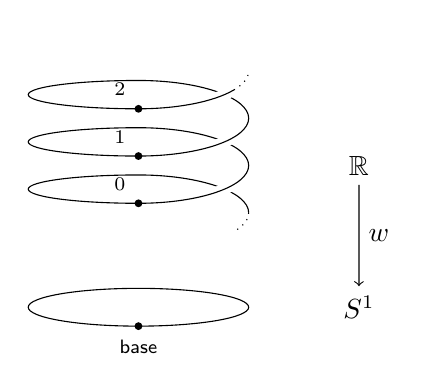
\begin{tikzpicture}[xscale=1.4,yscale=.6]
    \node (R) at (2,1) {$\mathbb{R}$};
    \node (S1) at (2,-2) {$S^1$};
    \draw[->] (R) -- node[auto] {$w$} (S1);
    \draw (0,-2) ellipse (1 and .4);
    \draw[dotted] (1,0) arc (0:-30:1 and .8);
    \draw (1,0) arc (0:90:1 and .8) arc (90:270:1 and .3) coordinate (t1);
    \draw[white,line width=4pt] (t1) arc (-90:90:1 and .8);
    \draw (t1) arc (-90:90:1 and .8) arc (90:270:1 and .3) coordinate (t2);
    \draw[white,line width=4pt] (t2) arc (-90:90:1 and .8);
    \draw (t2) arc (-90:90:1 and .8) arc (90:270:1 and .3) coordinate (t3);
    \draw[white,line width=4pt] (t3) arc (-90:90:1 and .8);
    \draw (t3) arc (-90:-30:1 and .8) coordinate (t4);
    \draw[dotted] (t4) arc (-30:0:1 and .8);
    \node[fill,circle,inner sep=1pt,label={below:\scriptsize \base}] at (0,-2.4) {};
    \node[fill,circle,inner sep=1pt,label={above left:\scriptsize 0}] at (0,.2) {};
    \node[fill,circle,inner sep=1pt,label={above left:\scriptsize 1}] at (0,1.2) {};
    \node[fill,circle,inner sep=1pt,label={above left:\scriptsize 2}] at (0,2.2) {};
  \end{tikzpicture}
  \caption{The winding map in classical topology}\label{fig:winding}
\end{figure}

Now in classical homotopy theory, where $\Sn^1$ is regarded as a topological space, we may proceed as follows.
\index{winding!map}%
Consider the ``winding'' map $w:\mathbb{R}\to \Sn ^1$, which looks like a helix projecting down onto the circle (see \cref{fig:winding}).
This map $w$ sends each point on the helix\index{helix} to the point on the circle that it is ``sitting above''.
It is a fibration, and the fiber over each point is isomorphic to the integers.\index{integers}
If we lift the path that goes counterclockwise around the loop on the bottom, we go up one level in the helix, incrementing the integer in the fiber.
Similarly, going clockwise around the loop on the bottom corresponds to going down one level in the helix, decrementing this count.
This fibration is called the \emph{universal cover} of the circle.
\index{universal!cover}%
\index{cover!universal}%
\index{covering space!universal}%

Now a basic fact in classical homotopy theory is that a map $E_1\to E_2$ of fibrations over $B$ which is a homotopy equivalence between $E_1$ and $E_2$ induces a homotopy equivalence on all fibers.
(We have already seen the type-theoretic version of this as well in \cref{thm:total-fiber-equiv}.)
Since $\mathbb{R}$ and $P_{\base} S^1$ are both contractible topological spaces, they are homotopy equivalent, and thus their fibers $\Z$ and $\Omega(\Sn ^1)$ over the basepoint are also homotopy equivalent.

\index{classical!homotopy theory|)}%

\subsection{The universal cover in type theory}
\label{sec:pi1s1-universal-cover}

\index{universal!cover|(}%
\index{cover!universal|(}%
\index{covering space!universal|(}%

Let us consider how we might express the preceding proof in type theory.
We have already remarked that the path fibration of $\Sn^1$ is represented by the type family $(x\mapsto (\base=x))$.
We have also already seen a good candidate for the universal cover of $\Sn^1$: it's none other than the type family $c:\Sn^1\to\type$ which we defined in \cref{sec:pi1s1-initial-thoughts}!
By definition, the fiber of this family over $\base$ is $\Z$, while the effect of transporting around $\lloop$ is to add one --- thus it behaves just as we would expect from \cref{fig:winding}.

However, since we don't know yet that this family behaves like a universal cover is supposed to (for instance, that its total space is simply connected), we use a different name for it.
For reference, therefore, we repeat the definition.
\index{integers}

\begin{defn}[Universal Cover of $\Sn^1$] \label{S1-universal-cover}
  Define $\code : \Sn ^1 \to \type$ by circle-recursion, with
  \begin{align*}
    \code(\base) &\defeq \Z \\
    \apfunc{\code}({\lloop}) &\defid \ua(\Zsuc).
  \end{align*}
\end{defn}

We emphasize briefly the definition of this family, since it is so different from how one usually defines covering spaces in classical homotopy theory.
To define a function by circle recursion, we need to find a point and a
loop in the codomain.  In this case, the codomain is $\type$, and the point
we choose is $\Z$, corresponding to our expectation that the
fiber of the universal cover should be the integers.  The loop we choose
is the successor/predecessor
\index{successor!isomorphism on Z@isomorphism on $\Z$}%
\index{predecessor!isomorphism on Z@isomorphism on $\Z$}%
isomorphism on $\Z$, which
corresponds to the fact that going around the loop in the base goes up
one level on the helix.  Univalence is necessary for this part of the
proof, because we need to convert a \emph{non-trivial} equivalence on $\Z$ into an identity.

We call this the fibration of ``codes'', because its elements are combinatorial data that act as codes for paths on the circle: the integer $n$ codes for the path which loops around the circle $n$ times.

From this definition, it is simple to calculate that transporting with
$\code$ takes $\lloop$ to the successor function, and
$\opp{\lloop}$ to the predecessor function:

\begin{lem} \label{lem:transport-s1-code}
\id{\transfib \code \lloop x} {x + 1} and
\id{\transfib \code {\opp \lloop} x} {x - 1}.
\end{lem}
\begin{proof}
For the first equation, we calculate as follows:
\begin{align}
{\transfib \code \lloop x}
&= \transfib {A \mapsto A} {(\ap{\code}{\lloop})} x \tag{by \cref{thm:transport-compose}}\\
&= \transfib {A \mapsto A} {\ua (\Zsuc)} x \tag{by computation for $\rec{\Sn^1}$}\\
&= x + 1 \tag{by computation for \ua}.
\end{align}
The second equation follows from the first, because $\transfib{B}{p}{\blank}$ and $\transfib{B}{\opp p}{\blank}$ are always inverses, so $\transfib\code {\opp \lloop}{\blank}$ must be the inverse of $\Zsuc$.
\end{proof}

We can now see what was wrong with our first approach: we defined $f$ and $g$ only on the fibers $\Omega(\Sn^1)$ and \Z, when we should have defined a whole morphism \emph{of fibrations} over $\Sn^1$.
In type theory, this means we should have defined functions having types
\begin{align}
  \prd{x:\Sn^1} &((\base=x) \to \code(x)) \qquad\text{and/or} \label{eq:pi1s1-encode}\\
  \prd{x:\Sn^1} &(\code(x) \to (\base=x))\label{eq:pi1s1-decode}
\end{align}
instead of only the special cases of these when $x$ is \base.
This is also an instance of a common observation in type theory: when attempting to prove something about particular inhabitants of some inductive type, it is often easier to generalize the statement so that it refers to \emph{all} inhabitants of that type, which we can then prove by induction.
Looked at in this way, the proof of $\Omega(\Sn^1)=\Z$ fits into the same pattern as the characterization of the identity types of coproducts and natural numbers in \cref{sec:compute-coprod,sec:compute-nat}.

At this point, there are two ways to finish the proof.
We can continue mimicking the classical argument by constructing~\eqref{eq:pi1s1-encode} or~\eqref{eq:pi1s1-decode} (it doesn't matter which), proving that a homotopy equivalence between total spaces induces an equivalence on fibers, and then that the total space of the universal cover is contractible.
The first type-theoretic proof of $\Omega(\Sn^1)=\Z$ followed this pattern; we call it the \emph{homotopy-theoretic} proof.

Later, however, we discovered that there is an alternative proof, which has a more type-theoretic feel and more closely follows the proofs in \cref{sec:compute-coprod,sec:compute-nat}.
In this proof, we directly construct both~\eqref{eq:pi1s1-encode} and~\eqref{eq:pi1s1-decode}, and prove that they are mutually inverse by calculation.
We will call this the \emph{encode-decode} proof, because we call the functions~\eqref{eq:pi1s1-encode} and~\eqref{eq:pi1s1-decode} \emph{encode} and \emph{decode} respectively.
Both proofs use the same construction of the cover given above.
Where the classical proof induces an equivalence on fibers from an equivalence between total spaces, the encode-decode proof constructs the inverse map (\emph{decode}) explicitly as a map between fibers.
And where the classical proof uses contractibility, the encode-decode proof uses path induction, circle induction, and integer induction.
These are the same tools used to prove contractibility --- indeed, path induction \emph{is} essentially contractibility of the path fibration composed with $\mathsf{transport}$ --- but they are applied in a different way.

Since this is a book about homotopy type theory, we present the encode-decode proof first.
A homotopy theorist who gets lost is encouraged to skip to the homotopy-theoretic proof (\cref{subsec:pi1s1-homotopy-theory}).

\index{universal!cover|)}%
\index{cover!universal|)}%
\index{covering space!universal|)}%

\subsection{The encode-decode proof}
\label{subsec:pi1s1-encode-decode}

\index{encode-decode method|(}%
\indexsee{encode}{encode-decode method}%
\indexsee{decode}{encode-decode method}%
We begin with the function~\eqref{eq:pi1s1-encode} that maps paths to codes:
\begin{defn}
Define $\encode : \prd{x : \Sn ^1} (\base=x) \rightarrow  \code(x)$ by
\[
\encode \: p \defeq \transfib{\code} p 0
\]
(we leave the argument $x$ implicit).
\end{defn}
Encode is defined by lifting a path into the universal cover, which
determines an equivalence, and then applying the resulting equivalence
to $0$.
The interesting thing about this function is that it computes a concrete
number from a loop on the circle, when this loop is represented using
the abstract groupoidal framework of homotopy type theory.  To gain an
intuition for how it does this, observe that by the above lemmas,
$\transfib \code \lloop x$ is the successor map and $\transfib \code {\opp
  \lloop} x$ is the predecessor map.
Further, $\mathsf{transport}$ is functorial (\cref{cha:basics}), so
$\transfib{\code} {\lloop \ct \lloop}{\blank}$ is
\[(\transfib \code \lloop-) \circ (\transfib \code \lloop-)\]
and so on.
Thus, when $p$ is a composition like
\[
\lloop \ct \opp \lloop \ct \lloop \ct \cdots
\]
$\transfib{\code}{p}{\blank}$ will compute a composition of functions like
\[
\Zsuc \circ \Zpred \circ \Zsuc \circ \cdots
\]
Applying this composition of functions to 0 will compute the
\index{winding!number}%
\emph{winding number} of the path --- how many times it goes around the
circle, with orientation marked by whether it is positive or negative,
after inverses have been canceled.  Thus, the computational behavior of
$\encode$ follows from the reduction rules for higher-inductive types and
univalence, and the action of $\mathsf{transport}$ on compositions and inverses.

Note that the instance $\encode' \defeq \encode_{\base}$ has type
$(\id \base \base) \rightarrow \Z$.
This will be one half of our desired equivalence; indeed, it is exactly the function $g$ defined in \cref{sec:pi1s1-initial-thoughts}.

Similarly, the function~\eqref{eq:pi1s1-decode} is a generalization of the function $\lloop^{\blank}$ from \cref{sec:pi1s1-initial-thoughts}.

\begin{defn}\label{thm:pi1s1-decode}
Define $\decode : \prd{x : \Sn ^1}\code(x) \rightarrow (\base=x)$ by
circle induction on $x$.  It suffices to give a function
${\code(\base) \rightarrow (\base=\base)}$, for which we use $\lloop^{\blank}$, and
to show that $\lloop^{\blank}$ respects the loop.
\end{defn}

\begin{proof}
To show that $\lloop^{\blank}$ respects the loop, it suffices to give a path
from $\lloop^{\blank}$ to itself that lies over $\lloop$.
By the definition of dependent paths, this means a path from
\[\transfib {(x' \mapsto \code(x') \rightarrow (\base=x'))} {\lloop} {\lloop^{\blank}}\]
to $\lloop^{\blank}$.  We define such a
path as follows:
\begin{align*}
  \MoveEqLeft \transfib {(x' \mapsto \code(x') \rightarrow (\base=x'))} \lloop {\lloop^{\blank}}\\
&= \transfibf {x'\mapsto (\base=x')}(\lloop) \circ {\lloop^{\blank}} \circ \transfibf \code ({\opp \lloop}) \\
&= (- \ct \lloop) \circ (\lloop^{\blank}) \circ \transfibf \code ({\opp \lloop}) \\
&= (- \ct \lloop) \circ (\lloop^{\blank}) \circ \Zpred \\
&= (n \mapsto \lloop^{n - 1} \ct \lloop).
\end{align*}
On the first line, we apply the characterization of $\mathsf{transport}$
when the outer connective of the fibration is $\rightarrow$, which
reduces the $\mathsf{transport}$ to pre- and post-composition with
$\mathsf{transport}$ at the domain and codomain types.  On the second line,
we apply the characterization of $\mathsf{transport}$ when the type family
is $x\mapsto \id{\base}{x}$, which is post-composition of paths.  On the third line,
we use the action of $\code$ on $\opp \lloop$ from
\cref{lem:transport-s1-code}.  And on the fourth line, we simply
reduce the function composition.  Thus, it suffices to show that for all
$n$, $\id{\lloop^{n - 1} \ct \lloop}{\lloop^{n}}$.  This is an easy application of \cref{thm:sign-induction}, using the groupoid laws.
\end{proof}

We can now show that $\encode$ and $\decode$ are quasi-inverses.
What used to be the difficult direction is now easy!

\begin{lem} \label{lem:s1-decode-encode}
For all $x: \Sn ^1$ and $p : \id \base x$, $\id
{\decode_x({{\encode_x(p)}})} p$.
\end{lem}

\begin{proof}
By path induction, it suffices to show that
\narrowequation{\id {\decode_{\base}({{\encode_{\base}(\refl{\base})}})} {\refl{\base}}.}
But
\narrowequation{\encode_{\base}(\refl{\base}) \jdeq \transfib{\code}{\refl{\base}} 0 \jdeq 0,}
and $\decode_{\base}(0) \jdeq \lloop^ 0 \jdeq \refl{\base}$.
\end{proof}

The other direction is not much harder.

\begin{lem} \label{lem:s1-encode-decode} For all
$x: \Sn ^1$ and $c : \code(x)$, we have $\id
{\encode_x({{\decode_x(c)}})} c$.
\end{lem}

\begin{proof}
The proof is by circle induction.  It suffices to show the case for
\base, because the case for \lloop is a path between paths in
$\Z$, which is immediate because $\Z$ is a set.

Thus, it suffices to show, for all $n : \Z$, that
\[
\id {\encode'(\lloop^n)} {n}.
\]
The proof is by induction, using \cref{thm:sign-induction}.
%
\begin{itemize}

\item In the case for $0$, the result is true by definition.

\item In the case for $n+1$,
\begin{align}
 {\encode'(\lloop^{n+1})}
&= {\encode'(\lloop^{n} \ct \lloop)} \tag{by definition of $\lloop^{\blank}$} \\
&= \transfib{\code}{(\lloop^{n} \ct \lloop)}{0} \tag{by definition of $\encode$}\\
&= \transfib{\code}{\lloop}{(\transfib{\code}{\lloop^n}{0})} \tag{by functoriality}\\
&= {(\transfib{\code}{\lloop^n}{0})} + 1 \tag{by \cref{lem:transport-s1-code}}\\
&= n + 1. \tag{by the inductive hypothesis}
\end{align}

\item The case for negatives is analogous.  \qedhere
\end{itemize}
\end{proof}

Finally, we conclude the theorem.

\begin{thm}
There is a family of equivalences $\prd{x : \Sn ^1} (\eqv {(\base=x)} {\code(x)})$.
\end{thm}

\begin{proof}
The maps $\encode$ and $\decode$ are quasi-inverses by
\cref{lem:s1-decode-encode,lem:s1-encode-decode}.
\end{proof}

\bibliographystyle{plain}
\bibliography{references}
\end{document}
